% \smalltitle{سوال 1.1}
% \begin{enumerate}
%     \item \phantom{text}
%     \\
%     \begin{latin}
%         \noindent
%         $S \rightarrow aSd|X|Y|Z$\\
%         $X \rightarrow aXc|Y$\\
%         $Y \rightarrow bYc|\epsilon$\\
%         $Z \rightarrow bZd|Y$
%     \end{latin}
%     \item \phantom{text}
%     \\
%     \begin{latin}
%         $S \rightarrow ab | Xb$\\
%         $X \rightarrow a|Y$\\
%         $Y \rightarrow aXb | bXa | aXa | bXb$
%     \end{latin}
% \end{enumerate}
ابتدا کد را نشان می‌دهیم و آنرا تحلیل می‌کنیم.
در این کد ابتدا تابع 
\lr{check\_schedulabe} 
فراخوانی می‌شود تا ببینیم اصلا می‌توان جدول را زمان‌بندی کرد یا خیر
\begin{center}
  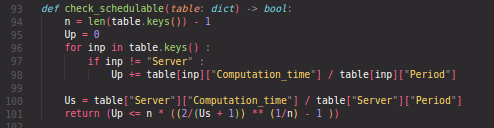
\includegraphics[scale=0.5]{pics/s1.png}
\end{center}
همانطور که می‌بینید، طبق فرمول گفته‌شده در اسلایدها، محاسبات را انجام می‌دهیم.

سپس تابع 
\lr{schedule\_EDF}
فراخوانی شده که عملا هر epoch 
زمانی یکبار می‌بیند که آیا تسک آپریودیکی وارد شده یا خیر و در صورتی که تسک وارد شده بود،‌ آنرا در لیست
انتظار سرور قرار می‌دهد تا هر وقت سرور شارژ شد، به اندازه شارژ خود و با اولویت خود تسک‌هایش را اجرا کند.
عکس زیر کد این قسمت را نشان می‌دهد.

\begin{center}
  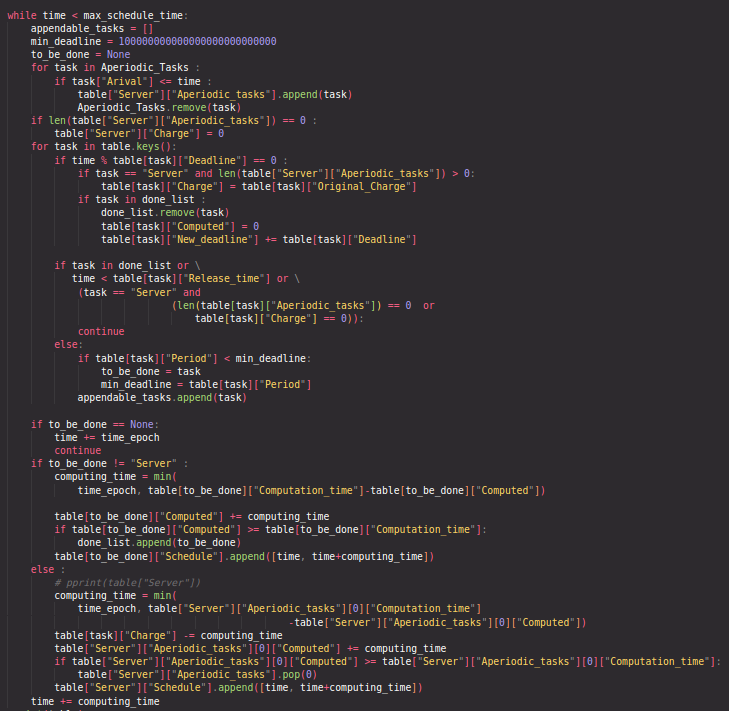
\includegraphics[scale=0.5]{pics/main.png}
\end{center}

در نهایت نیز با استفاده از تابع 
\lr{draw\_chart}
،
\lr{Gantt Chart}
مورد نظر را رسم می‌کنیم.
دو ورودی نمونه در خود برنامه تعریف شده‌اند که 
می‌توانید آنها را عوض کنید. 
ورودی‌های نمونه : 

\begin{center}
  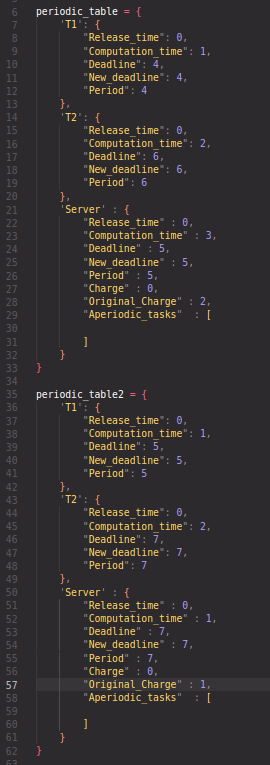
\includegraphics[scale=0.5]{pics/sample.png}
\end{center}
حال خروجی‌های متناظر هر کدام را مشاهده می‌کنیم.\\
خروجی اول :
\begin{center}
  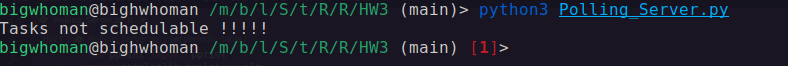
\includegraphics[scale=0.5]{pics/o1.png}
\end{center}
خروجی دوم : 
\begin{center}
  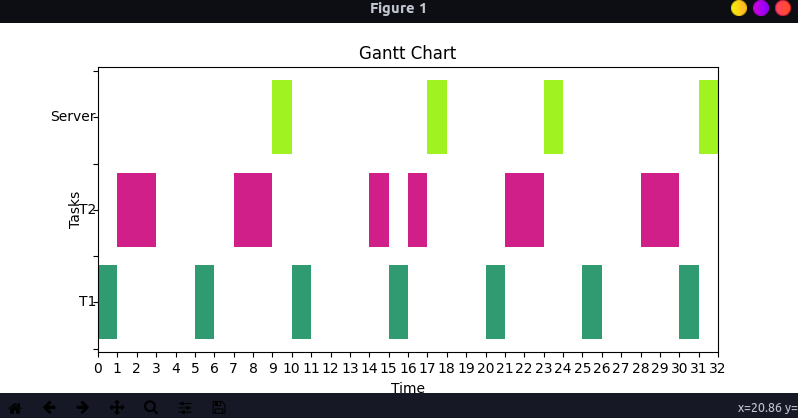
\includegraphics[scale=0.5]{pics/o2.png}
\end{center}

حال مشاهده کردید که ورودی اول طبق فرمول اسلایدها با زمان‌بندی RM قابل 
زمان‌بندی نیست اما ورودی دوم شروط لازم برای زمان‌بند‌پذیر بودن را دارا است.
% با معادلات بالا نیز می‌توان اثبات کرد 